\chapter{Introduction}
{
The Smart Energy Monitor is based on the concept of Non Intrusive Load Monitoring (NILM) which is a process for analyzing changes in the voltage and current going into a house and deducing what appliances are used in the house as well as their individual energy consumption. Electric meters with NILM technology are used by utility companies to survey the specific uses of electric power in different homes. NILM is considered a low-cost alternative to attaching individual monitors on each appliance. 

The system can measure both reactive power and real power. Hence two appliances with the same total power draw can be distinguished by differences in their complex impedance. For example, a refrigerator electric motor and a pure resistive heater can be distinguished in part because the electric motor has significant changes in reactive power when it turns on and off, whereas the heater has almost none.

NILM systems can also identify appliances with a series of individual changes in power draw. These appliances are modeled as finite state machines. A dishwasher, for example, has heaters and motors that turn on and off during a typical dish washing cycle. These will be identified as clusters, and power draw for the entire cluster will be recorded. Hence ``dishwasher'' power draw can be identified as opposed to ``resistor heating unit'' and ``electric motor''.
Thus designing a energy monitoring unit using this NLIM has many benefits. The overview of the system is as follow:
\begin{figure}[H]
	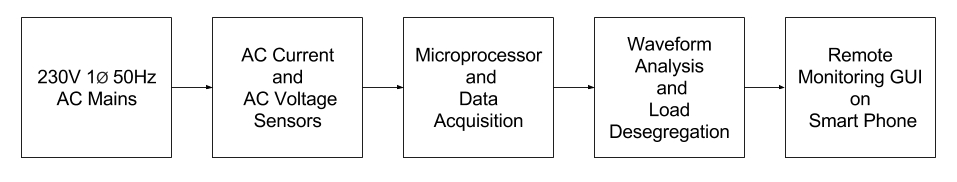
\includegraphics[scale=0.5]{introblockdia} % first figure itself
	\caption{Basic Block diagram of the System}
	\label{blck}
\end{figure}
}
%--------------------------------------------------------------------
% \LaTeX users - skip the section below
%-------------------------------------------------------------------


%--------------------------------------------------------------------------

\section {Motivation}
How many planets would it take to support our lifestyle? As blunt as it may sound, the truth stands unchanged, staring at the face of the unknown future of the whole planet. It didn't take us long to open our hearts (and homes) to the amazing changes that technology brought into our lives. Amidst the ease and comfort, everything else seems to be collateral damage to us now. One such commodity is electricity.Electricity consumption rates from non renewable sources of energy is increasing at an alarming rate by the hour. Our increasing dependency on these replenishing  sources calls for innovative ways to tap on our consumption rates, preferably on a daily basis. Electrical appliances used on a daily basis are monitored ambiguously, hence an increase in the prices may not be found. 
The outcome of this project, the Smart Energy Monitor is aimed to help the average Indian consumer monitor their appliance usage on a daily basis hence keep track of their consumption.

\section{Objectives}
\begin{enumerate}
	\item To disaggregate load appliances using minimum hardware & efficient and accurate classification algorithms.
	\item To provide the user with Real-time monitoring and alerts on their smartphone.
	\item To track the power consumption of individual load appliances and provide the user with an estimate of their monthly electricity bill.
\end{enumerate}